
\subsection{Esempi numerici trasformate fratte}
\subsubsection{Poli distinti}
Sia la seguente funzione razionale fratta con due poli distinti: $p_1 = -2$,
$p_2=-5$, $n=2,\ m=1,\ n-m=1$
$$
F(s) = \frac{s-10}{(s+2)(s+5)} = \frac{R_1}{s+2} + \frac{R_2}{s+5}
$$

Si calcolano i residui polari:
$$\begin{aligned}
R_1 &= \lim_{s\to -2} (s+2)F(s) = \lim_{s\to -2} \frac{s-10}{s+5} =
\frac{-12}{+3} = -4\\
R_2 &= \lim_{s\to -5} (s+5)F(s) = \lim_{s\to -5}
\frac{s-10}{s+2} = \frac{-15}{-3} = 5\\
\sum_{i=1}^2R_i &= \frac{b_m}{a_n} = \frac{1}{1} \Rightarrow R_2 = 1-R_1
\end{aligned}
$$
L'antitrasformata:
$$
f(t) = \Lap^{-1}[F(s)] = \Lap^{-1}\left[-\frac{4}{s+2}+\frac{5}{s+5}\right] =
\left(-4e^{-2t} + 5e^{-5t}\right)\delta_{-1}(t)
$$

In alternativa alla tecnica dei residui si può sfruttare il principio di
identità dei polinomi
$$\begin{aligned}
F(s) &= \frac{s-10}{(s+2)(s+5)} = \frac{R_1}{s+2} + \frac{R_2}{s+5} =
\frac{R_1(s+5)+R_2(s+2)}{(s+2)(s+5)} =\\
&=\frac{(R_1+R_2)s+(5R_1+2R_2)}{(s+2)(s+5)} \Rightarrow \left\{
\begin{aligned}
R_1+R_2 &=1\\
5R_1+2R_2 &= -10
\end{aligned}\right. = \ldots \\&=
\left\{\begin{aligned}
R_1 &= -4 \\ R_2 &= 5
\end{aligned}\right.
\end{aligned}$$

Analogamente è possibile sostituire $n$ valori differenti di $s$ e risolvere il
sistema ottenuto per ricavare i residui.

\newpage
\subsubsection{Radici coincidenti}
La seguente funzione ha due poli
$$
\left[\begin{aligned}
p_1 &= 0\\
p_2 &= -3 \qquad m_a=2\\
n-m &=2
\end{aligned}\right.
$$
$$
F(s) = \frac{s+18}{s(s+3)^2} = \frac{R_1}{s} + \frac{R_2^{(1)}}{s+3} +
\frac{R_2^{(2)}}{(s+3)^2}
$$
Si calcolano i residui
$$\begin{aligned}
R_1 &= \lim_{s\to 0} sF(s) = \lim_{s\to 0} \frac{s+18}{(s+3)^2} = \frac{18}{9}
= 2\\
R_2^{(2)} &= \lim_{s\to -3} (s+3)^2 F(s) =
\lim_{s\to -3} \frac{s+18}{s} = \frac{15}{-3} = -5\\
R_2^{(1)} &\stackrel{n-m>1}{=} -\sum_{\begin{aligned}
i&=1\\ i &\neq 2
\end{aligned}}^2 R_i = -R_1 = -2 \qquad \text{oppure}\\
R_2^{(1)} & = \lim_{s\to -3} \frac{d}{ds} \left[(s+3)^2F(s)\right] = -2
\end{aligned}$$
Nella sommatoria vanno calcolati solo i residui semplici e non quelli associati
a potenze superiori all'unità.

$$
f(t) = \Lap^{-1}\left[F(s)\right] = \Lap^{-1} \left[\frac{2}{s} +
\frac{-2}{s+3} + \frac{-5}{(s+3)^2}\right] =
\left(2-2e^{-3t} -5e^{-3t}\cdot t\right)\delta_{-1}(t)
$$

\newpage
\subsection{Radici complesse e coniugate}
$$
F(s) = \frac{100}{(s+1)(s^2 + 4s + 13)}
$$
I poli saranno $p_1 = -1,\ p_2 = -2+j3,\ p_3 = p_2^* = -2-j3 $\\
La decomposizione in fratti semplici
$$
F(s) = \frac{R_1}{s+1} + \frac{R_2}{s+2-j3} + \frac{R_3=R_2^*}{s+2+j3}
$$
$$\begin{aligned}
R_1 &= \lim_{s\to -1} (s+1)F(s) = \lim_{s\to -1}\frac{100}{s^2+4s +13} =
\frac{100}{10} = 10\\
R_2 &= \lim_{s\to -2+j3} (s+2-j3)F(s) =\lim_{s\to -2+j3}
\frac{100}{(s+1)(s+2+j3)} = \\
&=\frac{100}{(-2 + j3 + 1)(\cancel{-2}+j3 \cancel{+
2} + j3)} = -\frac{5}{3}(3-j) = -5 + \frac{5}{3}j=R_3^*\\
R_3 &= -5 - \frac{5}{3}j
\end{aligned}$$
Si può dunque antitrasformare
$$\begin{aligned}
f(t) &= \Lap^{-1} [f(s)] = \Lap^{-1}
\left[
\frac{10}{s+1} - \frac{5}{3}\left(
\frac{3-j}{s+2-j3}+ \frac{3+j}{s+2+j3}
\right)
\right] = \\
&=10\left(e^{-t} -\frac{1}{6}\cdot
2|R_2|e^{\Re(p_2)t}\cos\left(\Im(p_2)\cdot t + \text{arg}(p_2)\right)
\right) = \\
&= 10\left(e^{-t} -\frac{1}{6}2\sqrt{10}e^{-2t} \cos(3t+
\text{arg}(-3+j))\right)\delta_{-1}(t)
\end{aligned}$$

In alternativa sfruttando il principio di identità dei polinomi
$$
F(s) = \frac{100}{(s+1)(s^2 + 4s + 13)} = \frac{R_1}{s+1} +
\frac{R_as+R_b}{s^2+4s+13}
$$
Si calcola $R_1=10$ con la formula precedente, si esegue il minimo comune
multiplo
$$
100 = 10(s^2+4s + 13)+(s+1)(R_as+R_b)
$$
In questo caso può essere conveniente sostituire due valori di $s$
$$
\begin{aligned}
s=0 &\rightarrow\\
s=1 &\rightarrow
\end{aligned}
\left\{
\begin{aligned}
 100 &= 130 + R_b\\
 100 &= 180 + 2(R_a + R_b)
\end{aligned}\right.
\rightarrow
\left\{
\begin{aligned}
R_a &= -10\\
R_b &= -30
\end{aligned}
\right.
$$

\newpage
Si può calcolare l'antitrasformata
$$
f(t) = \Lap^{-1} [F(s)] = \Lap^{-1} \left[
\frac{10}{s+1} -10\frac{s+3}{(s+2)^2+9}
\right]
$$
Il secondo termine può essere antitrasformato facendo comparire il $3$ ed
$(s+2)$ in modo da far comparire le trasformate notevoli di seno e coseno.
$$
\frac{s+3  }{(s+2)^2 + 9}  =\frac{(s+2)+1}{(s+2)^2 + 3^2}
$$
$$\begin{aligned}
f(t) &=
\Lap^{-1}\left[\frac{10}{s+1}-10\frac{s+2}{(s+2)^2+3^2}-\frac{10}{3}\frac{3
} {(s+2)^2 +3^2} \right] =\\
&= 10\left(e^{-t} -e^{-2t} \left( \cos(3t)+\frac{1}{3}\sin(3t) \right)
\right)\delta_{-1}(t)
\end{aligned}$$
Con varie formule trigonometriche è possibile ottenere l'espressione identica
alla precedente $\sqrt{10}\cos(3t+
\text{arg}(-3+j))$.

\newpage
\section{Funzione di trasferimento}
Strumento molto utile al fine di calcolare le risposte forzate dei sistemi.
Si consideri un sistema Lineare tempo-invariante
$S$, sottoposto ad un  ingresso $u(t)$ con uscita $y(t)$.

La definizione di \textit{funzione di trasferimento} non è univoca, si
definisce in questo corso come la trasformata della matrice delle risposte
impulsive.
$$
W(s) \stackrel{\text{def}}{=}\Lap\left[W(t)\right]
$$
Non sono presenti informazioni riguardo lo stato del sistema nella matrice
$W(t)$, per la biunivocità della trasformata, anche la funzione di
trasferimento non conterrà informazioni circa lo stato del sistema.

Si considera un ingresso generico $u(t)$, viene \textit{campionato} con una
sequenza di impulsi rettangolari di periodo $T$.
Si ottiene dunque una rappresentazione $\tilde{u}(t)$
$$
\tilde{u}(t) = \sum_{i=0}^{+\infty}\delta_T(t-iT)Tu(iT)
$$

\begin{figure}[h]
\centering
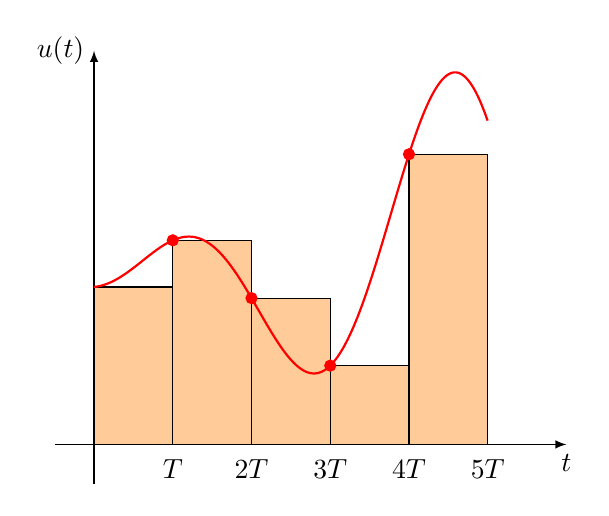
\begin{tikzpicture}[scale=1,declare
function={f(\x)=(0.5*\x*sin(100*\x)+2+0.1*\x;}]
\coordinate (start) at (0,{f(0)});
\coordinate (x0) at (1,{f(1)});
\coordinate (x1) at (2,{f(2)});
\coordinate (x2) at (3,{f(3)});
\coordinate (x3) at (4,{f(4)});
\coordinate (x4) at (5,{f(5)});
\coordinate (end) at (5.0,{f(5.0)});
\draw[fill=orange!40!white] (0,0) rectangle (1,{f(0)});
\draw[fill=orange!40!white] (1,0) rectangle (2,{f(1)});
\draw[fill=orange!40!white] (2,0) rectangle (3,{f(2)});
\draw[fill=orange!40!white] (3,0) rectangle (4,{f(3)});
\draw[fill=orange!40!white] (4,0) rectangle (5,{f(4)});
%\draw (5,0)--(5,{f(5)});
\draw [-latex] (-0.5,0) -- (6,0) node (xaxis) [below] {$t$};
\draw [-latex] (0,-0.5) -- (0,5) node [left] {$u(t)$};
\foreach \x/\xtext in {1/T ,2/2T, 3/3T , 4/4T , 5/5T }
 \draw[xshift=\x cm] (0pt,3pt) -- (0pt,0pt)
node[below=2pt,fill=white,font=\normalsize]
  {$\xtext$};
\draw[domain=0:5,samples=200,variable=\x,red,thick] plot ({\x},{f(\x)});

\foreach \n in {0,1,2,3}
\draw[red,fill=red] (x\n) circle (2pt) node[font=\normalsize] {$ $};
%\draw[<->] (2,-1)--(3,-1) node[above,midway] {$\Delta x$};
\end{tikzpicture}
\end{figure}

Essendo il sistema lineare per ipotesi, l'uscita sarà combinazione
lineare delle singole risposte ai differenti impulsi rettangolari
$$
\tilde{y}(t) = \sum_{i=0}^{+\infty} W_T(t-iT)Tu(iT)
\stackrel{}T\to 0{\longrightarrow} y_f(t) =
\int_0^{+\infty} W(t-\tau)u(\tau)d\tau
$$
Si può estendere l'estremo di integrazione inferiore dato che $u(\tau)$ è nulla
per $\tau<0$
$$
y_f(t) = \int_{-\infty}^{+\infty}W(t-\tau)u(\tau)d\tau = W(t)*u(t)
$$
La risposta forzata di un sistema LTI è sempre data dal prodotto di
convoluzione tra la matrice delle risposte agli impulsi e l'ingresso.

Si applica la trasformata di Laplace della risposta forzata
$$
\Lap[y_f(t)] = Y_f(s) = \Lap[W(t)*u(t)] = \Lap[W(t)]\cdot \Lap[u(t)] = W(s)
\cdot U(s)
$$
Se il sistema è \textit{SISO} (Single-Input-Single-Output) allora
$$
W(s) = \frac{Y_f(s)}{U(s)}
$$
Con la funzione di trasferimento non è necessario eseguire l'integrale di
convoluzione per determinare l'uscita forzata ma è sufficiente eseguire il
prodotto delle due trasformate e antitrasformare.

%\subsubsection{Esempio}
Sia la seguente ISU generica
$$
\left\{\begin{aligned}
\dot{x} &= Ax+Bu \\
y &= Cx +Du
\end{aligned}\right.
$$
Il movimento forzato
$$
x_f(t) = \int_0^t e^{A(t-\tau)} Bu(\tau)d\tau
\stackrel{u=\delta}{\longrightarrow} x_\delta(t) =
\int_0^te^{A(t-\tau)}B\delta(\tau)d\tau = e^{At} B = H(t)
$$
Uscita forzata
$$
y_f(t) = Cx_f(t) +Du(t) \stackrel{u=\delta}{\longrightarrow} y_\delta(t) =
Ce^{At}B + D\delta(t) = W(t)
$$
In alternativa
$$
y_f(t) =C\int_0^t e^{A(t-\tau)} Bu(\tau) d\tau + Du(t) = \int_0^t
\left(Ce^{A(t-\tau)}B + D\delta(t-\tau)\right)u(\tau)d\tau
$$
Si estendono gli estremi di integrazione
$$
y_f(t) = \int_{-\infty}^{+\infty} W(t-\tau)u(\tau)d\tau
\stackrel{\text{def}}{=} W(t)*u(t)
$$

\subsubsection{Esempio nastro trasportatore}
Sia dato un nastro di lunghezza $L$ avvolto su due rulli che ruotano con
velocità costante $v$, sul nastro viene depositata una certa quantità di
materiale $u(t)$.

Il nastro non altera la quantità di materiale, dunque l'uscita sarà
semplicemente l'ingresso traslato nel tempo di una quantità $\tau=\frac{L}{v}$
$$
y(t) = u\left(t-\frac{L}{v}\right) = u(t-\tau)
$$

Per calcolare la ISU è necessario definire una variabile di stato che ne
caratterizzi la condizione iniziale, ossia la quantità di materiale depositata
lungo il nastro, funzione dello spazio $s$ e del tempo $t$.
Il sistema è dunque a parametri \textit{distribuiti} perché ha uno stato che
varia con continuità ed ha quindi infiniti valori differenti.
Il modello ISU non sarà più alle derivate totali ma alle derivate parziali.

Se si sottopone il sistema ad un ingresso impulsivo si ottiene la risposta
all'impulso e trasformando si ottiene anche la funzione di trasferimento
$$
u(t) = \delta(t) \Rightarrow w(t) = \delta(t-\tau)
\stackrel{\Lap}{\longrightarrow} W(s) = e^{-s\tau}
$$
La funzione di trasferimento non è in questo caso legata all'esistenza di una
ISU in forma canonica, è sufficiente che il sistema sia
lineare-tempo-invariante.
L'uscita è ancora il prodotto di convoluzione tra la funzione di trasferimento
e l'ingresso.

\subsubsection{Definizione funzione di trasferimento con ISU}
Si applica la trasformata di Laplace all'intero sistema ISU
$$
\left\{\begin{aligned}
\dot{x} &= Ax+Bu \\
y &= Cx +Du
\end{aligned}\right. \stackrel{\Lap}{\longrightarrow} \left\{\begin{aligned}
sX(s) - x(0) &= AX(s) + BU(s) \\
Y(s) &= CX(s) + DU(s)
\end{aligned}\right.
$$
Raccogliendo i termini della prima equazione
$$
\left(sI-A\right)X(s) = x(0) + BU(s)
$$
La matrice $(sI-A)$ è invertibile per tutti i valori di $s$ ad eccezione degli
autovalori della matrice $A$.
Con tale ipotesi:
$$\left\{\begin{aligned}
X(s) &= (sI-A)^{-1}x(0) + (sI-A)^{-1}BU(s)\\
Y(s) &= C(sI-A)^{-1}x(0) + \left(C(sI-A)^{-1}B+D\right)U(s)\end{aligned}\right.
$$
Si è ricavata una ISU in forma esplicita, analoga alle formule di Lagrange
ricavate alla sezione \ref{sec:formule_lagrange}.
Per analogia
$$
\left\{\begin{aligned}
X(s) &= X_l(s) + X_f(s)\\
Y(s) &= Y_l(s) + Y_f(s)
\end{aligned}\right.
$$

Si ottiene ancora la funzione di trasferimento
$$
W(s) = C(sI-A)^{-1}B + D
$$

L'evoluzione libera
$$\begin{aligned}
x_l(t) = e^{At}x_0 \stackrel{\Lap}{\longleftrightarrow}& X_l(s) =
(sI-A)^{-1}x(0) \qquad \forall x(0)\\
&\Downarrow\\
\Lap[e^{At}] = \Lap[\Phi(t)] &= (sI-A)^{-1}=\Phi(s)
\end{aligned}
$$
La trasformata della matrice esponenziale è l'inversa di $(sI-A)$, è possibile
calcolare la matrice esponenziale come la sua antitrasformata. Analogamente è
comodo calcolare la risposta in evoluzione libera.

La matrice delle risposte impulsive nello stato
$$\begin{aligned}
H(t) &= e^{At} B \stackrel{\Lap}{\longleftrightarrow} H(s) = (sI-A)^{-1}B
=\Phi(s)B\\
x_f(t) &= \int_0^t H(t-\tau)u(\tau)d\tau = H(t)*u(t)
\stackrel{\Lap}{\longleftrightarrow} X_f(s) =H(s)U(s)
\end{aligned}
$$

Analogamente per l'uscita
$$\begin{aligned}
y_l(t) &= Ce^{At}x(0) \stackrel{\Lap}{\longleftrightarrow} Y_l(s) =
C(sI-A)^{-1}x(0)\\
y_f(t) &= C\int_0^te^{A(t-\tau)}Bu(\tau) + Du(t) d\tau
\stackrel{\Lap}{\longleftrightarrow} Y_f(s) = W(s)U(s)
\end{aligned}$$
